\section{Περιγραφή Λειτουργίας Μετασχηματιστών Υποβιβασμού}

\subsection{Μετατροπέας υποβιβασμού}

\noindent
Μετασχηματιστής Υποβιβασμού είναι μία συσκευή η οποία έχει ως βασική λειτουργία την (παραγωγή) τάσης εξόδου η οποία είναι μειωμένη σε σχέση με την τάση εισόδου.  
\begin{figure}[h]
	\centering
	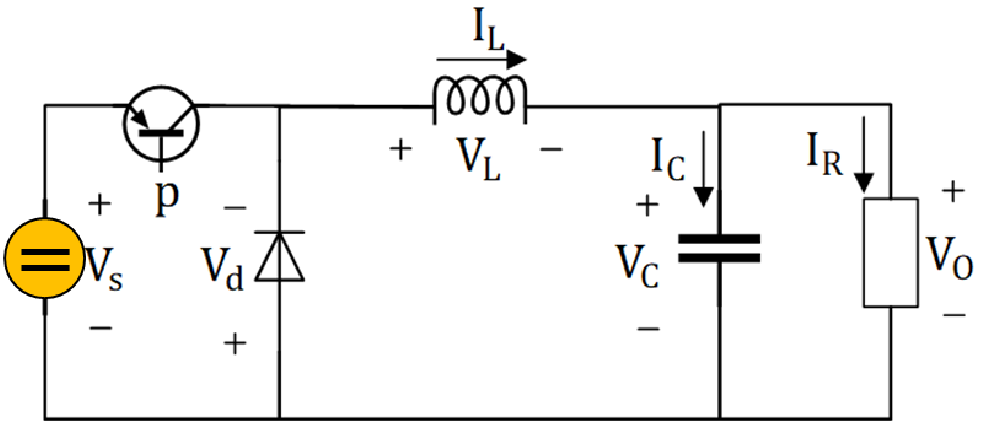
\includegraphics[width=0.37\textwidth]{Images/buckConverter.png}
\end{figure}

\noindent
Η μείωση της τάσης επιτυγχάνεται μέσω της δημιουργίας τετραγωνικών παλμών συγκεκριμένου πλάτους με αποτέλεσμα την αυξομείωση της τάσης αρκετά γρήγορα ώστε η μέση τιμή της τάσης εξόδου να είναι μικρότερη από την τάση εισόδου. 

\noindent\\
O τετραγωνικός παλμός δημιουργείται ανοιγοκλείνοντας τον διακόπτη εφαρμόζοντας συγκριμένη τάση σε αυτόν ενώ πέραν αυτού, χρησιμοποιείται μία δίοδος ?????????????????????????????? ??????????????????????? ????????????????? ??????????????? ???????, ένα πηνίο για την εξομάλυνση του ρεύματος εξόδου και ένας πυκνωτής για την εξομάλυνση της τάσης εξόδου. 
Τέλος, η χρήση του διακόπτη δημιουργεί δύο φάσεις λειτουργία ανάλογα την κατάστασή του.
\noindent\\\\
\textbf{Κλειστός διακόπτης (Φ1)}
\begin{figure}[h]
	\centering
	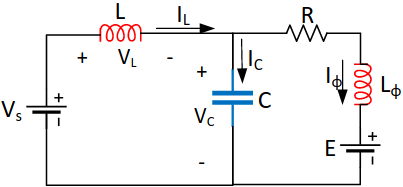
\includegraphics[width=0.35\textwidth]{Images/Phase_1}
\end{figure}

\noindent
Κατά την φάση Φ1, εφαρμόζεται κατάλληλη τιμή τάσης στον διακόπτη και έτσι αντικαθίσταται με βραχυκύκλωμα. Ως αποτέλεσμα, η δίοδος ανακυκλώνεται καθώς είναι ανάστροφα πολωμένη εφόσον στην άνοδό της πηγής συνδέεται το αρνητικό άκρο της πηγής και στην κάθοδο το θετικό. Ακόμη, μέσω του πηνίου ρέει ρεύμα προς το φορτίο και προς τον πυκνωτή με αποτέλεσμα την φόρτιση του.  ??????????????????????????

\noindent\\
Για την επίλυση του συστήματος είναι απαραίτητο να οριστούν οι μεταβλητές εισόδου και εξόδου.  Ως μεταβλητές εισόδου ορίζονται η τάση εισόδου ($V_s$) και η τάση στο φορτίο ($E$) ενώ ως μεταβλητές εισόδου ορίζονται τα ρεύματα των πηνίων ($I_L$ και $Ι_{\Phi}$) και η τάση του πυκνωτή ($V_C$). Επιπλέον, είναι απαραίτητο να βρεθούν οι πίνακες A, B, C και D ώστε να επιλυθεί το εξής σύστημα:
\begin{align}
	\dot{X} = A\cdot X + B\cdot U \label{x_dot}\\
	Y = C \cdot X + D \cdot U \label{y}
\end{align} 

\noindent
Οι πίνακες προκύπτουν εφαρμόζοντας νόμο τάσεων του Kirchhoff στον κόμβο Α:
\begin{align}
											V_L = L \cdot \frac{dI_L(t)}{dt} = V_s - V_c &\xRightarrow{} \frac{dI_L (t)}{dt} = - \frac{1}{L} \cdot V_c + \frac{1}{L} \cdot V_s\\
											\notag \\
	V_c - I_{\Phi} \cdot R - \frac{dIL_{\Phi}}{dt} \cdot L_{\Phi} - E = 0 &\xRightarrow{}  \frac{dIL_{\Phi}}{dt} = -\frac{R}{L_{\Phi}} \cdot I_{\Phi} + \frac{1}{L_{\Phi}} \cdot V_c - \frac{1}{L_{\Phi}} \cdot E
\end{align}

και εφαρμόζοντας νόμο ρευμάτων του Kirchhoff στον κόμβο Α προκύπτει η εξής σχέση:
\begin{equation}
	I_L = I_c + I_{\Phi} \xRightarrow{} \frac{dV_c}{dt} \cdot C = I_L - I_{\Phi} \xRightarrow{} \frac{dV_c}{dt} = \frac{1}{C} \cdot I_L - \frac{1}{C} \cdot I_{\Phi}
\end{equation}

\clearpage
\noindent
Επιλύοντας τις σχέσεις σε μορφή πινάκων σύμφωνα με τις σχέσεις (\ref{x_dot}) και (\ref{y}) προκύπτουν τα εξής συστήματα:
 \begin{equation*}
 	\overbrace{
	 	\frac{d}{dt} 
	 	\begin{bmatrix}
	 		I_L\\
	 		I_{\Phi}\\
	 		V_c
	 	\end{bmatrix}
	 }^{\dot{X}}
 	=
 	\overbrace{
	 	\begin{bmatrix}
						0 		& 					0 			 & -\frac{1}{L}\\
			            0       & -\frac{R}{L_{\Phi}} & \frac{1}{L_{\Phi}}\\
			\frac{1}{C}  & 		   -\frac{1}{C}      & 				0
	 	\end{bmatrix}
	 }^A
 	\cdot
 	\overbrace{
	 	\begin{bmatrix}
			I_L\\
			I_{\Phi}\\
			V_c
		\end{bmatrix}
	}^X
	+ 	
	\overbrace{
		\begin{bmatrix}
			 \frac{1}{L}  &	    			0 			\\
					0           &  -\frac{1}{L_{\Phi}}\\
					0		    & 		  			0
		\end{bmatrix}
	}^B
	\cdot
	\overbrace{
		\begin{bmatrix}
			V_s\\
			E		
		\end{bmatrix}
	}^U
\end{equation*} 

\begin{equation*}
	\underbrace{
		\begin{bmatrix}
			I_L\\
			I_{\Phi}\\
			V_c
		\end{bmatrix}
	}_Y
	=
	\underbrace{
		\begin{bmatrix}
			1 & 0 & 0\\
			0 & 1 & 0\\
			0 & 0 & 1
		\end{bmatrix}
	}_C
	\cdot
	\underbrace{
		\begin{bmatrix}
			I_L\\
			I_{\Phi}\\
			V_c
		\end{bmatrix}
	}_X
	+ 
	\underbrace{	
		\begin{bmatrix}
			0 & 0 \\
			0 & 0 \\
			0 & 0
		\end{bmatrix}
	}_D
	\cdot
	\underbrace{
		\begin{bmatrix}
			V_s\\
			E		
		\end{bmatrix}
	}_U
\end{equation*}
\clearpage
\subsection{Ελεγχόμενος μετατροπέας υποβιβασμού}